\iffalse\documentclass{article}\fi
\documentclass[12pt]{article}

\usepackage{sbc-template}
\usepackage{graphicx,url}

\usepackage[english]{babel}   
\usepackage[utf8]{inputenc} 

\usepackage{graphicx}

\usepackage{etoolbox}
\patchcmd{\thebibliography}{\section*{\refname}}{}{}{}

\graphicspath{ {./images/} }

     
\sloppy

\title{Segmentation and Image Crop using SLICO Superpixels and Hierarchy of Partitions}

\author{Felipe Augusto Lima Reis\inst{1}}

\address{PUC Minas - Pontifícia Universidade Católica de Minas Gerais
  \email{falreis@sga.pucminas.br} }

\begin{document} 

\maketitle

\begin{abstract}
  This paper presents a approach to use SLICO superpixels with hierarchy of partitions to segmentation and automatic crop of images, to speed up image edition and treatment. The algorithm uses a data tree to link regions to merge. Also, it can provide automatic segmentation or follow users instructions. This approachs also uses reinforced learning to learn user preferences criteria to segmentation and merge regions.
\end{abstract}
     
\begin{resumo} 
  Este artigo apresenta uma proposta para utilização superpixels SLICO e hierarquia de partições para segmentação e corte automático de imagens, a fim de facilitar a edição e o tratamento das mesmas. O algoritmo utiliza uma árvore de dados para estabelecer relações entre duas ou mais regiões a serem fundidas, possibilitando a fusão automática de partições ou seguindo orientação do usuário. A proposta ainda utiliza uma rede neural utilizando \textit{reinforced learning} a fim de aprender os critérios preferidos do usuário para segmentação e união das regiões.
\end{resumo}


\section{Introdução} \label{sec:introducao}



\section{Referencial Teórico} \label{sec:ref_teorico}

The first page must display the paper title, the name and address of the
authors, the abstract in English and ``resumo'' in Portuguese (``resumos'' are
required only for papers written in Portuguese). The title must be centered
over the whole page, in 16 point boldface font and with 12 points of space
before itself. Author names must be centered in 12 point font, bold, all of
them disposed in the same line, separated by commas and with 12 points of
space after the title. Addresses must be centered in 12 point font, also with
12 points of space after the authors' names. E-mail addresses should be
written using font Courier New, 10 point nominal size, with 6 points of space
before and 6 points of space after.

The abstract and ``resumo'' (if is the case) must be in 12 point Times font,
indented 0.8cm on both sides. The word \textbf{Abstract} and \textbf{Resumo},
should be written in boldface and must precede the text.

\section{Materiais e Métodos} \label{sec:mat_metodos}


\section{Testes, Resultados e Discussões} \label{sec:testes}

Section titles must be in boldface, 13pt, flush left. There should be an extra
12 pt of space before each title. Section numbering is optional. The first
paragraph of each section should not be indented, while the first lines of
subsequent paragraphs should be indented by 1.27 cm.

\subsection{Subsections}

The subsection titles must be in boldface, 12pt, flush left.

\section{Figures and Captions}\label{sec:figs}


Figure and table captions should be centered if less than one line
(Figure~\ref{fig:exampleFig1}), otherwise justified and indented by 0.8cm on
both margins, as shown in Figure~\ref{fig:exampleFig2}. The caption font must
be Helvetica, 10 point, boldface, with 6 points of space before and after each
caption.

\begin{figure}[ht]
\centering
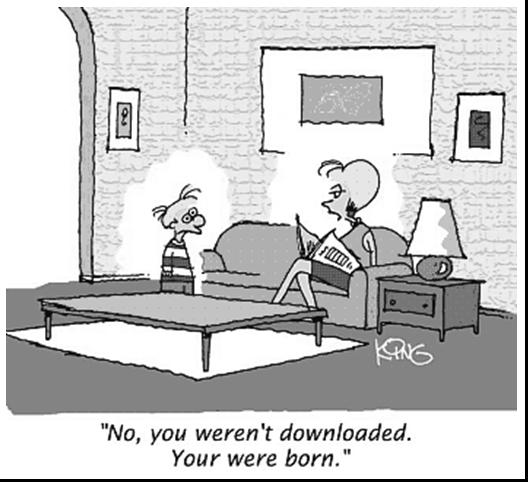
\includegraphics[width=.5\textwidth]{fig1.jpg}
\caption{A typical figure}
\label{fig:exampleFig1}
\end{figure}

\begin{figure}[ht]
\centering
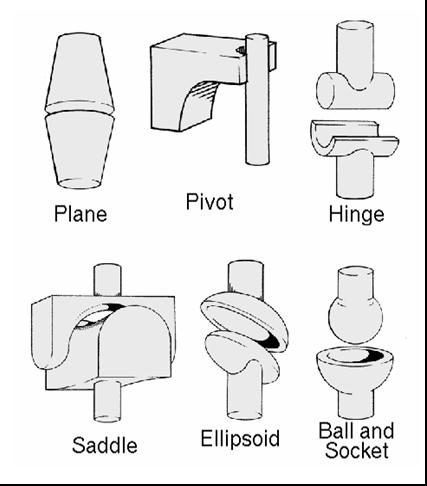
\includegraphics[width=.3\textwidth]{fig2.jpg}
\caption{This figure is an example of a figure caption taking more than one
  line and justified considering margins mentioned in Section~\ref{sec:figs}.}
\label{fig:exampleFig2}
\end{figure}

In tables, try to avoid the use of colored or shaded backgrounds, and avoid
thick, doubled, or unnecessary framing lines. When reporting empirical data,
do not use more decimal digits than warranted by their precision and
reproducibility. Table caption must be placed before the table (see Table 1)
and the font used must also be Helvetica, 10 point, boldface, with 6 points of
space before and after each caption.

\begin{table}[ht]
\centering
\caption{Variables to be considered on the evaluation of interaction
  techniques}
\label{tab:exTable1}
\smallskip
\begin{tabular}{|l|c|c|}
\hline
& Value 1 & Value 2\\[0.5ex]
\hline
&&\\[-2ex]
Case 1 & 1.0 $\pm$ 0.1 & 1.75$\times$10$^{-5}$ $\pm$ 5$\times$10$^{-7}$\\[0.5ex]
\hline
&&\\[-2ex]
Case 2 & 0.003(1) & 100.0\\[0.5ex]
\hline
\end{tabular}
\end{table}

\section{Conclusão} \label{sec:conclusao}

All images and illustrations should be in black-and-white, or gray tones,
excepting for the papers that will be electronically available (on CD-ROMs,
internet, etc.). The image resolution on paper should be about 600 dpi for
black-and-white images, and 150-300 dpi for grayscale images.  Do not include
images with excessive resolution, as they may take hours to print, without any
visible difference in the result. 

\section{Referências} \label{sec:referencias}

\bibliographystyle{sbc}
\bibliography{sbc-template}

\end{document}
